\documentclass[xcolor=table]{beamer}

\mode<presentation> {
  \usetheme{CambridgeUS}
}
\usecolortheme{seahorse}
\setbeamertemplate{navigation symbols}{}
\setbeamertemplate{caption}[numbered]

\usepackage{graphicx} % Allows including images
\usepackage{booktabs} % Allows the use of \toprule, \midrule and \bottomrule in tables

\usepackage[utf8]{inputenc}
\usepackage[T2A]{fontenc}
\usepackage[english,russian]{babel}
\usepackage{listings}
\usepackage{xcolor}
\usepackage{caption}
\usepackage{stmaryrd}

\usepackage{appendixnumberbeamer}

%\usepackage{textpos}

\usepackage{biblatex}

\bibliography{main2.bib}

\setbeamertemplate{itemize items}[circle]
\setbeamertemplate{enumerate items}[circle]

\newcommand{\citepres}[1]{{\it \citetitle{#1}}, \citeauthor{#1}, \citeyear{#1}}

\renewcommand{\footnotesize}{\tiny}

\titlegraphic{
\includegraphics[height=3cm,width=3cm]{logo.png}\hspace{1cm}}
\title[Университет ИТМО]{Применение метода суперкомпиляции для специализации реляционных программ}

\author{Куклина Мария Дмитриевна}
\institute[]
{
Университет ИТМО\\ 
\vspace{0.3cm}
Научный руководитель: к.ф.-м.н. Близнец Иван Александрович\\
%\vspace{0.2cm}
Научный консультант: Вербицкая Екатерина Андреевна
%2020
}
\date[]{2020 г.}


%\addtobeamertemplate{frametitle}{}{%
%\begin{textblock*}{100mm}(.85\textwidth,-1cm)
%
\includegraphics[height=2cm,width=2cm]{logo.png}
%\end{textblock*}}


\begin{document}

\begin{frame}[noframenumbering,plain]
\titlepage
\end{frame}

%
% TODO: footnote цвет более серый

%%%%%%%%%%%%%%%%%%%%%%%%%%%%%%%%%%%%%%%%%%%%%%%%%%%
%
%
%%%%%%%%%%%%%%%%%%%%%%%%%%%%%%%%%%%%%%%%%%%%%%%%%%%
%\begin{frame}{Реляционное программирование}
%\begin{block}{Определение}
%    Вид декларативного программирования, в котором программы представляются как набор отношений между аргументами.
%\end{block}
%\vspace{0.7cm}
%\begin{block}{Пример}
%   Пример {\it запросов} для отношения ``меньше или равно'' $\text{leq}^o \subseteq \text{Int} \times \text{Int}$:
%   \begin{itemize}
%   \item $\text{leq}^o\text{(1, 2)}$ --- проверка корректности отношения.
%   \item $\text{leq}^o\text{(X, Y)}$ --- поиск значений X и Y, при которых отношение выполняется.
%   \end{itemize}
%%  Пример {\it запросов} для отношения умножения $\text{mul}^o \subseteq \text{Int} \times \text{Int} \times \text{Int}$:
%%  \begin{itemize}
%%    \item $\texttt{mul}^o(\texttt{2, 2, 4})$ --- проверка корректности отношения.
%%    \item $\texttt{mul}^o(\texttt{2, 2, C})$ --- поиск всех \texttt{С}, таких что \texttt{2 * 2 = C}.
%%    \item $\texttt{mul}^o(\texttt{A, 1, 4})$ --- поиск всех \texttt{A}, таких что \texttt{A * 1 = 1}.
%%    \item $\texttt{mul}^o(\texttt{A, B, C})$ --- поиск всех троек \texttt{A, B, С}, таких что \texttt{A * B = C}.
%%  \end{itemize}
%\end{block}
%\end{frame}
%%%%%%%%%%%%%%%%%%%%%%%%%%%%%%%%%%%%%%%%%%%%%%%%%%%
%
%
%%%%%%%%%%%%%%%%%%%%%%%%%%%%%%%%%%%%%%%%%%%%%%%%%%%
\begin{frame}{Реляционное программирование}
  \begin{block}{Реляционное программирование}
      Вид декларативного программирования, в котором программы
      представляются как набор математических отношений.
  \end{block}
   \vspace{0.4cm}
   \begin{block}{}
   Пример запросов для отношения ``меньше или равно'' $\text{leq}^o \subseteq \text{Int} \times \text{Int}$:
   \begin{itemize}
   \item $\text{leq}^o\text{(1, 2)}$ --- проверить, что отношение 1 $\leq$ 2 выполняется. % найти все значения X, такие что 1 $\leq$ X.
   \item $\text{leq}^o\text{(X, Y)}$ --- поиск всех значений X и Y, таких что X $\leq$ Y.
   \end{itemize}
   \end{block}

\end{frame}

\begin{frame}{miniKanren}
  \begin{block}{miniKanren}
    Встраиваемый предметно-ориентированный язык реляционного
    программирования,
    представленный как набор операторов, которые нужно реализовать
    в хостовом языке\footnotemark.
  \end{block}\footnotetext{\citepres{byrdMK}}
  \vspace{0.5cm}
  % {\bf Применение}
  % \begin{itemize}
  % \item Легковесная логическая подсистема проекта.
  % \item Поиск лечения редких генетических заболеваний в точной медицине\footnote{\citepres{medMK}}.
  % \item Генерация программ по спецификации входов и выходов на основе \emph{реляционного интерпретатора}.
  % \item Порождение решения задач поиска по решению задачи распознавания\footnote{\citepres{lozov}}.
  % \end{itemize}

  \begin{block}{Преимущества}
  \begin{itemize}
  \item Одно отношение можно применять для решения связанных задач. 
  \item Реализует {\it полный поиск}: гарантируется, что каждый ответ будет со временем найден.
  \end{itemize}
  \end{block}

  %{\bf Важное преимущество}
  %\begin{itemize}
  %%\item Одно отношение можно применять для решения нескольких связанных задач.
  %\item Полнота поиска: гарантируется, что все ответы будут найдены.
  %%\item Чистота: 
  %% Что такое обратимость языковых конструкций?
  %%\item Минималистичный язык с простой реализацией.
  %\end{itemize}

\end{frame}
%%%%%%%%%%%%%%%%%%%%%%%%%%%%%%%%%%%%%%%%%%%%%%%%%%%
%
%
%%%%%%%%%%%%%%%%%%%%%%%%%%%%%%%%%%%%%%%%%%%%%%%%%%%
\begin{frame}{Постановка проблемы}

\begin{itemize}
%\item Сложность реализации эффективных программ.
\item Реализовывать эффективные программы сложно.
\item Производительность запроса сильно зависит от того,
      значения каких компонент отношения нужно найти.
%   Пример {\it запросов} для отношения ``меньше или равно'' $\text{leq}^o \subseteq \text{Int} \times \text{Int}$:

% Многие отношения на деле являются функциональными, из-за чего запуск в ``обратном'' направлении очень неэффективен.\\
% Поиск входов по выходам отношения работает значительно медленнее, чем ``прямой'' запуск.
% {\bf Примеры}
% \begin{itemize}
% \item Программы, порождённые инструментом по трансляции из функционального языка в miniKanren\footnote{\citepres{trconv}}.
% \item Порождение решения задач поиска.
% \end{itemize}
\end{itemize}
\end{frame}
%%%%%%%%%%%%%%%%%%%%%%%%%%%%%%%%%%%%%%%%%%%%%%%%%%%
%
%%%%%%%%%%%%%%%%%%%%%%%%%%%%%%%%%%%%%%%%%%%%%%%%%%%
\begin{frame}{Специализация}
\begin{block}{Определение}
Автоматизированная техника оптимизации программ, при которой из программы удаляются
избыточные вычисления, зависимые от частично известного входа\footnotemark.
\end{block}\footnotetext{\citepres{jones}}

\begin{itemize}
\item Частичная дедукция --- класс методов специализации для логический языков, в частности, для Prolog.\footnote{\citepres{advanced}}
\item Специализация miniKanren на основе \emph{конъюнктивной частичной дедукции (CPD)}\footnote{\citepres{lozov}}:
\begin{itemize}
\item %Сложна в поддержке,
      даёт нестабильные результаты;
\item предоставляет библиотеку для построения специализаторов.
\end{itemize}
\end{itemize}
\end{frame}
%%%%%%%%%%%%%%%%%%%%%%%%%%%%%%%%%%%%%%%%%%%%%%%%%%%
%
%%%%%%%%%%%%%%%%%%%%%%%%%%%%%%%%%%%%%%%%%%%%%%%%%%%
\begin{frame}{Суперкомпиляция}

\begin{block}{Определение}
Техника автоматической трансформации и анализа программ, при которой
программа символьно исполняется с сохранением истории вычислений, на основе
которой принимаются решения об оптимизации.
\end{block}

\begin{itemize}
\item Суперкомпиляторы применяются во основном для функциональных языков\footnote{\citepres{scPos}}.
%\item % Суперкомпиляция показывает хорошие результаты при специализации.
%      Суперкомпиляция позволяет достичь не более чем линейного ускорения\footnote{\citepres{scompRevisited}}
\item Существует полуавтоматическая суперкомпиляция для Prolog\footnote{\citepres{apropos}}.
\item Имеются теоретические доводы в пользу автоматической суперкомпиляции для \text{Prolog}\footnote{\citepres{scompRevisited}}. %^{\text{9}}$.
\end{itemize}

\end{frame}
%%%%%%%%%%%%%%%%%%%%%%%%%%%%%%%%%%%%%%%%%%%%%%%%%%%
%
%
%%%%%%%%%%%%%%%%%%%%%%%%%%%%%%%%%%%%%%%%%%%%%%%%%%%
\begin{frame}{Цели и задачи}
\begin{block}{Цель}
Улучшение результатов специализации реляционных программ путём применения метода суперкомпиляции.
\end{block}
%%%%%%%%%%%%%%%%%%%%%%%%%%%%%%%%%%%%%%%%%%%%%%%%%%%
%
%
%%%%%%%%%%%%%%%%%%%%%%%%%%%%%%%%%%%%%%%%%%%%%%%%%%%
\begin{block}{Задачи}
\begin{itemize}
\item Реализовать суперкомпилятор для miniKanren.
\item Рассмотреть возможные методы улучшения получившегося суперкомпилятора.
\item Протестировать суперкомпилированные программы и сравнить их
      c получившимися в результате применения CPD и c оригинальными.
\end{itemize}
\end{block}
\end{frame}


%%%%%%%%%%%%%%%%%%%%%%%%%%%%%%%%%%%%%%%%%%%%%%%%%%%
%
%
%%%%%%%%%%%%%%%%%%%%%%%%%%%%%%%%%%%%%%%%%%%%%%%%%%%
% \begin{frame}{$\mu$Kanren}
% \begin{block}{Определение}
% Минимальное подмножество miniKanren, содержащее в себе только основные операции языка:
% конъюнкция, дизъюнкция,
% унификация, введение свежей переменной и вызов реляционного отношения.\\
% \end{block}
% \begin{itemize}
% \item Программа на $\mu$Kanren представляет собой логическую формулу, атомы которой --- это либо унификация двух термов, либо вызов отношения.
% \item Не содержит операторов miniKanren c эффектами. 
% \item Библиотека для специализации работает с $\mu$Kanren\footnote{\url{https://github.com/kajigor/uKanren_transformations}}.
% \end{itemize}
% \end{frame}

%%%%%%%%%%%%%%%%%%%%%%%%%%%%%%%%%%%%%%%%%%%%%%%%%%%
%
%
%%%%%%%%%%%%%%%%%%%%%%%%%%%%%%%%%%%%%%%%%%%%%%%%%%%
\begin{frame}{Суперкомпиляция для miniKanren}

\begin{figure}[h!]
\center
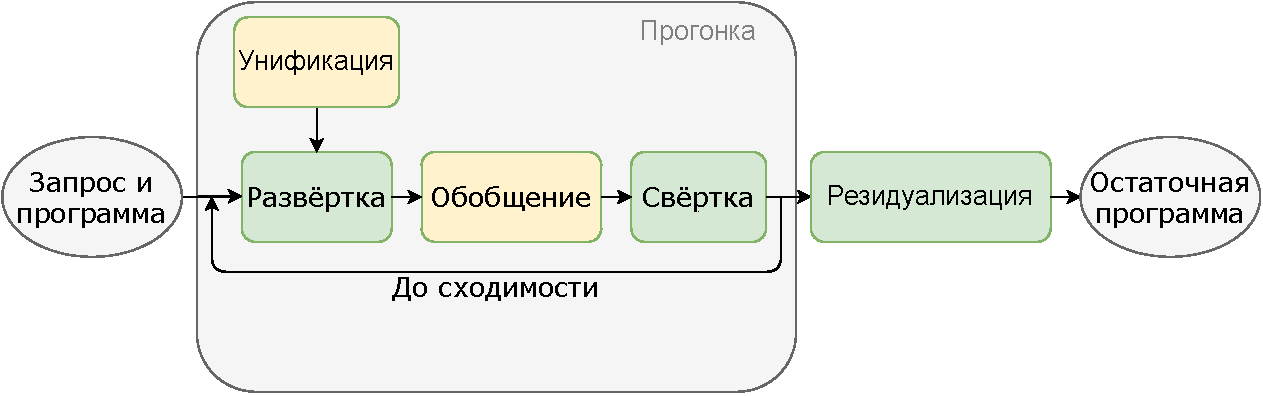
\includegraphics[scale=0.55]{scompflow.pdf}
\caption{
    Схема алгоритма суперкомпиляции\\
}
\label{fig:scomp}
\end{figure}
{\footnotesize
\begin{tabular}{l}

\includegraphics[scale=0.4]{orange.pdf} --- библиотека по специализации miniKanren c дополнениями\\

\includegraphics[scale=0.4]{green.pdf} --- собственная разработка
\end{tabular}
}


%В процессе суперкомпиляции строится корневой ориентированный граф, описывающий историю символьного исполнения,
%из которого извлекается \emph{остаточная} программа --- специализированная версия исходной.

\end{frame}

\begin{frame}{Особенности miniKanren для реализации развёртки}
\begin{block}{}
{\bf Развёртка} определяет шаг символьного вычисления,
на котором порождается множество возможных состояний программы.
\end{block}
\vspace{0.5cm}
\begin{block}
{\bf Значимые особенности}
\begin{itemize}
\item Существует несколько возможных способов реализации развёртки.
\item Допускается переупорядочивание элементов выражения.
% \item Реляционность предполагает, что методы специализации логических
%\item Допускает больше возможностей для суперкомпиляции, чем другие языки.
\end{itemize}
\end{block}
\end{frame}

\begin{frame}{Результаты задачи}
\begin{itemize}
\item Реализован базовый алгоритм суперкомпиляции.
%\begin{itemize}
%\item Развёртка рассматривает все возможные состояния.
%\item Используемый алгоритм обобщения основан на алгоритме для конъюнктивной частичной дедукции,
%      для которого доказана терминируемость.
% \item Стратегия вычисления соответствует семантике языка.
%\end{itemize}
\item Разработан и реализован алгоритм построения оптимизированной программы по графу суперкомпиляции.
\end{itemize}
\end{frame}

\begin{frame}{Улучшение суперкомпиляции для miniKanren}
\begin{block}{Проблемы}
\begin{itemize}
\item Стратегия свёртки приводит к повторению символьных вычислений.
\item Классическое использование обобщения может приводить к избыточным вычислениям.
\item Тривиальная стратегия вычисления порождает слишком много ветвей исполнения.
\item Реализованный суперкомпилятор поддерживает лишь базовый
      набор операторов miniKanren; поддержка расширений может
      потребовать более сложный алгоритм.
\end{itemize}
\end{block}
\end{frame}

\begin{frame}{Результаты задачи}
\begin{itemize}
\item Применены подходы по улучшению алгоритма суперкомпиляции.
\begin{itemize}
\item Добавлено кэширование.
\item Реализованы модификации обобщения.
\item Проанализированы и реализованы допустимые стратегии вычисления.
\end{itemize}
\item Библиотека расширена оператором неравенства:
      это наиболее полезное расширение miniKanren\footnote{\citepres{diseqSem}}.
     %наиболее важным расширением
     % miniKanren --- оператором неравенства
\item Реализовано расширение суперкомпилятора, учитывающее информацию о неравенствах термов.
%\item Расширение неравенствами библиотеки для специализации.
%\item Расширение суперкомпилятора, учитывающее информацию о неравенствах.
\end{itemize}
\end{frame}

%%%%%%%%%%%%%%%%%%%%%%%%%%%%%%%%%%%%%%%%%%%%%%%%%%%
%
%%%%%%%%%%%%%%%%%%%%%%%%%%%%%%%%%%%%%%%%%%%%%%%%%%%
\begin{frame}{Тестирование}

\begin{description}[leftmargin=!]
\item[Реализация miniKanren:] проект OCanren\footnote{\url{https://github.com/JetBrains-Research/OCanren}}\\
\item[Реализация CPD для miniKanren:] проект uKanren\_transformations\footnote{\url{https://github.com/kajigor/uKanren_transformations/}}
\item[Реализация CPD для Prolog:] проект ECCE\footnote{\url{https://github.com/leuschel/ecce}}
\item[Платформа:] Intel Core i5-6200U CPU, 2.30GHz, DDR4, 12GiB.
\end{description}
{\bf Сценарий}
\begin{enumerate}
\item Суперкомпиляция тестовой программы.
\item Трансляция остаточной программы в OCanren.
\item Замер времени исполнения.
\item Сравнение времени исполнения с оригинальной программой и результатами
      применения CPD.
\end{enumerate}
\end{frame}
%%%%%%%%%%%%%%%%%%%%%%%%%%%%%%%%%%%%%%%%%%%%%%%%%%%
%
%%%%%%%%%%%%%%%%%%%%%%%%%%%%%%%%%%%%%%%%%%%%%%%%%%%
\begin{frame}{Программы для тестирования}
\begin{description}
\item[sort]Алгоритм реляционной сортировки.\\
      % Запрос: $\text{sort}^o$ xs ys.
      {\bf Запрос}: сортировка случайного списка длины 50.
\item[isPath] Проверка принадлежности пути графу.\\
      % {\bf Запрос}: $\text{isPath}^o$ p g true.
      {\bf Запрос}: поиск  произвольного пути длины 10, принадлежащих графу c 21 вершиной и 50 рёбрами.
\item[logint] Реляционный интерпретатор формул логики высказываний.\\
      {\bf Запрос}: поиск 1000 истинных формул в данной подстановке.
      % {\bf Запрос}: $\text{logint}^o$ s q true.
\item[lam] Реляционный интерпретатор лямбда-выражений.\\
      % {\bf Запрос}: $\text{lam}^o$ q q.
      {\bf Запрос}: поиск n термов, редуцирующиеся к указанной форме.
% \item Реляционный алгоритм вывода типов для просто типизированного лямбда-исчисления.
%\item[a] Реляционный интерпретатор подмножества Scheme.
\end{description}
\end{frame}
%%%%%%%%%%%%%%%%%%%%%%%%%%%%%%%%%%%%%%%%%%%%%%%%%%%
%
%%%%%%%%%%%%%%%%%%%%%%%%%%%%%%%%%%%%%%%%%%%%%%%%%%%
\begin{frame}{Сравнение улучшений}

\begin{itemize}
\item Были рассмотрены 5 модификаций базового алгоритма
      c 8 стратегиями развертки:
      \begin{itemize}
      \item 1 модификация описана в статьях;
      \item 4 модификации предложены мной.
      \end{itemize}
\item Все модификации улучшают работу оригинального суперкомпилятора.
\item Систематически модификация, описанная в статьях, давала
      результат лучше или не сильно хуже, чем остальные модификации.
\item По результатам исследования была выявлена
      лучшая стратегия развёртки.
\end{itemize}

\end{frame}
%%%%%%%%%%%%%%%%%%%%%%%%%%%%%%%%%%%%%%%%%%%%%%%%%%%
%
%%%%%%%%%%%%%%%%%%%%%%%%%%%%%%%%%%%%%%%%%%%%%%%%%%%
\begin{frame}
    {Сравнение суперкомпиляторов с существующими решениями}
\begin{table}
\center
\begin{tabular}{|c|c|c|c|c|c|}
\hline
{\it Параметр} & {\it Оригинал} & {\it ECCE }  & {\it CPD} & {\bf Б.С.} & {\bf М.С.} \\ \hline
\rowcolor{black!10}
{\bf sort} & \multicolumn{5}{|l|}{случайный список фиксированной длины } \\ \hline
50       & 8.42     & 12.28 & 13.2 & {\bf 0.239} & 0.242 \\ \hline

\rowcolor{black!10}
 {\bf isPath} & \multicolumn{5}{|l|}{поиск 10 путей} \\ \hline
  граф 3      & > 300 & {\bf 1.03} & 1.19 & 2.43 & 1.81 \\ \hline
\rowcolor{black!10}
 {\bf isPath} & \multicolumn{5}{|l|}{произвольный путь длины 10} \\ \hline
 граф 1  &  12.51  & 1.01 & 1.20 & 1.28 &  {\bf 0.48} \\
 граф 2  &  > 300s & 1.73 & 2.09 & 0.85 & {\bf 0.48} \\ 
 %граф 3  &         & 9.90 & 12.73& 3.29 & {\bf 1.23} \\
 \hline

\rowcolor{black!10}
{\bf logint} & \multicolumn{5}{|l|}{генерация логических формул} \\ \hline
без переменных & > 300    & 0.17  & 2.7  & - & {\bf 0.11} \\
одна переменная&          & 0.09  & 1.7  & - & {\bf 0.07} \\
%2 &          & 0.08   & 0.9  & -  & {\bf 0.05} \\
\hline

\rowcolor{black!10}
{\bf lam} & \multicolumn{5}{|l|}{термы в нормальной форме} \\ \hline
%10 термов к себе    & 0.17     & 0.001 & 0.008 & 0.002  \\
50 термов & > 300    & 2.98  & 0.08 & 0.08 & {\bf 0.04}   \\
%1000 термов к const & 1.01     & 0.126 & 0.263 & 0.274  \\
\hline
\end{tabular}
\caption{Время исполнения программ для данных специализаторов, cекунды}
\label{fig:totalResult}
\end{table}
\end{frame}

%%%%%%%%%%%%%%%%%%%%%%%%%%%%%%%%%%%%%%%%%%%%%%%%%%%
%
%%%%%%%%%%%%%%%%%%%%%%%%%%%%%%%%%%%%%%%%%%%%%%%%%%%
\begin{frame}{Результаты работы}
  \begin{itemize}
  \item Реализован и протестирован суперкомпилятор.
  \item Применены подходы по улучшению качества суперкомпиляции.
  \item Добавлены неравенства в библиотеку для специализации.
  % \item Реализованы реляционные интерпретаторы для тестирования.
  % \item Проведено тестирование и анализ результатов.
  \item Исправлены баги библиотеки для специализации.
\item Работа была представлена на воркшопе по трендам логического программирования TEASE-LP'20.
\item Ссылка на репозиторий: \url{https://github.com/RehMaar/uKanren-spec}
  \end{itemize}
\end{frame}

%\begin{frame}{Спасибо за внимание!}
%\begin{itemize}
%\item Работа была представлена на воркшопе по трендам логического программирования TEASE-LP'20.
%\item Ссылка на репозиторий: \url{https://github.com/RehMaar/uKanren-spec}
%\end{itemize}
%\end{frame}


% Доп. слайды.
% Пример специализации.
\appendix
\begin{frame}[plain]
\center
{\large Дополнительные слайды}
\end{frame}

\begin{frame}{Пример сравнения модификаций суперкомпилятора}
\begin{table}[h!]
\center
\begin{tabular}{|p{2.3cm}||c|c|c|c|c|c|}
\hline
                 & \multicolumn{6}{|l|}{Вариации суперкомпиляторов} \\ \hline
Стратегии развёртки &{\it Б.С.}&{\it М.1}&{\it М.2}&{\it М.3}&{\it M.4}&{\it M.5} \\ \hline \hline
{\it Full        }&    -        &    -        & 0.078       & 0.062      &    -        & - \\ \hline
{\it Full-non-rec}& 0.137       & 0.040       & 0.093       & 0.042      & 0.069       & {\bf 0.040} \\ \hline
{\it Seq         }& 0.086       & 0.082       & 0.066       & 0.049      & {\bf 0.050} & {\bf 0.041} \\ \hline
{\it Non-rec     }& 0.043       & {\bf 0.031} & 0.063       & 0.044      & 0.055       & 0.046 \\ \hline
{\it Rec         }& {\bf 0.037} & 0.034       & {\bf 0.045} & 0.040      & 0.051       & 0.049 \\ \hline
{\it Min         }& {\bf 0.037} & 0.039       & 0.049       & 0.041      & 0.054       & 0.045 \\ \hline
{\it Max         }& 0.068       & 0.070       & 0.067       &{\bf 0.036} & 0.062       & 0.071 \\ \hline
{\it First       }& 0.104       & 0.100       & 0.110       & 0.095      & 0.137       & 0.073 \\ \hline
\end{tabular}
\caption{Время исполнения запроса к \lstinline{logint} для генерации формул с двумя переменными, секунды.}
\label{fig:logintTest3}
\end{table}
\end{frame}

\begin{frame}
Условные обозначения для стратегий развёртывания:
\begin{itemize}
\item {\it Full} и {\it Full-non-rec} обозначают полную стратегию и полную стратегию развёртывания с приоритетом на нерекурсивные вызовы соответственно;
\item {\it Seq} обозначает последовательную стратегию развёртывания;
\item {\it Non-rec} и {\it Rec} обозначают нерекурсивную и рекурсивную стратегии соответственно;
\item {\it Min} и {\it Max} обозначают минимальную и максимальную стратегии соответственно;
\item {\it First} обозначает стратегию, при которой всегда развёртывается первый конъюнкт.
\end{itemize}
\end{frame}

\begin{frame}
Условные обозначения для модификаций:
\begin{itemize}
\item {\it Б.С.} обозначает базовый суперкомпилятор с обобщением вниз на предков;
\item {\it М.1 } обозначает модификацию, при которой происходит запрет на обобщение сразу после обобщения;
\item {\it M.2 } обозначает модификацию, при которой обобщение происходит на все ранее вычисленные вершины;
\item {\it M.3 } обозначает модификацию, при которой происходит обобщение вверх на родительские вершины;
\item {\it M.4 } обозначает модификацию, при которой происходит обобщение вверх на родительские вершины, кроме корневой.
\item {\it M.5 } обозначает модификацию, при которой происходит обобщение вверх на родительские вершины, а также запрет обобщения после обобщения.
\end{itemize}
\end{frame}

\begin{frame}{Граф конфигураций для программы конкатенации трёх списков doubleAppend}
\center
\includegraphics[scale=0.3]{./tree.png}
\end{frame}
\end{document} 
